%%%%%%%%%%%%%%%%%%%%%%%%%%%%%%%%
%% What is an event? 
%%%%%%%%%%%%%%%%%%%%%%%%%%%%%%%%

At the LHC we define an \textit{event} as everything that happens in a proton bunch crossing.
These high energy collisions are very complex, often resulting in the production of many hundreds of
particles. An illustration of this complexity is shown in Fig.~\ref{fig:event_full_event}.
A proper description of what happens is impeded by the composite nature of the proton, and by the
strong coupling constant of QCD, the quantum field theory governing hadron
interactions.
Fortunately, it turns out that the full process can be factorized into independent subprocesses,
each taking place at different energy scales~\cite{Skands:2011pf}. 


\begin{figure}[htpb]
  \centering
  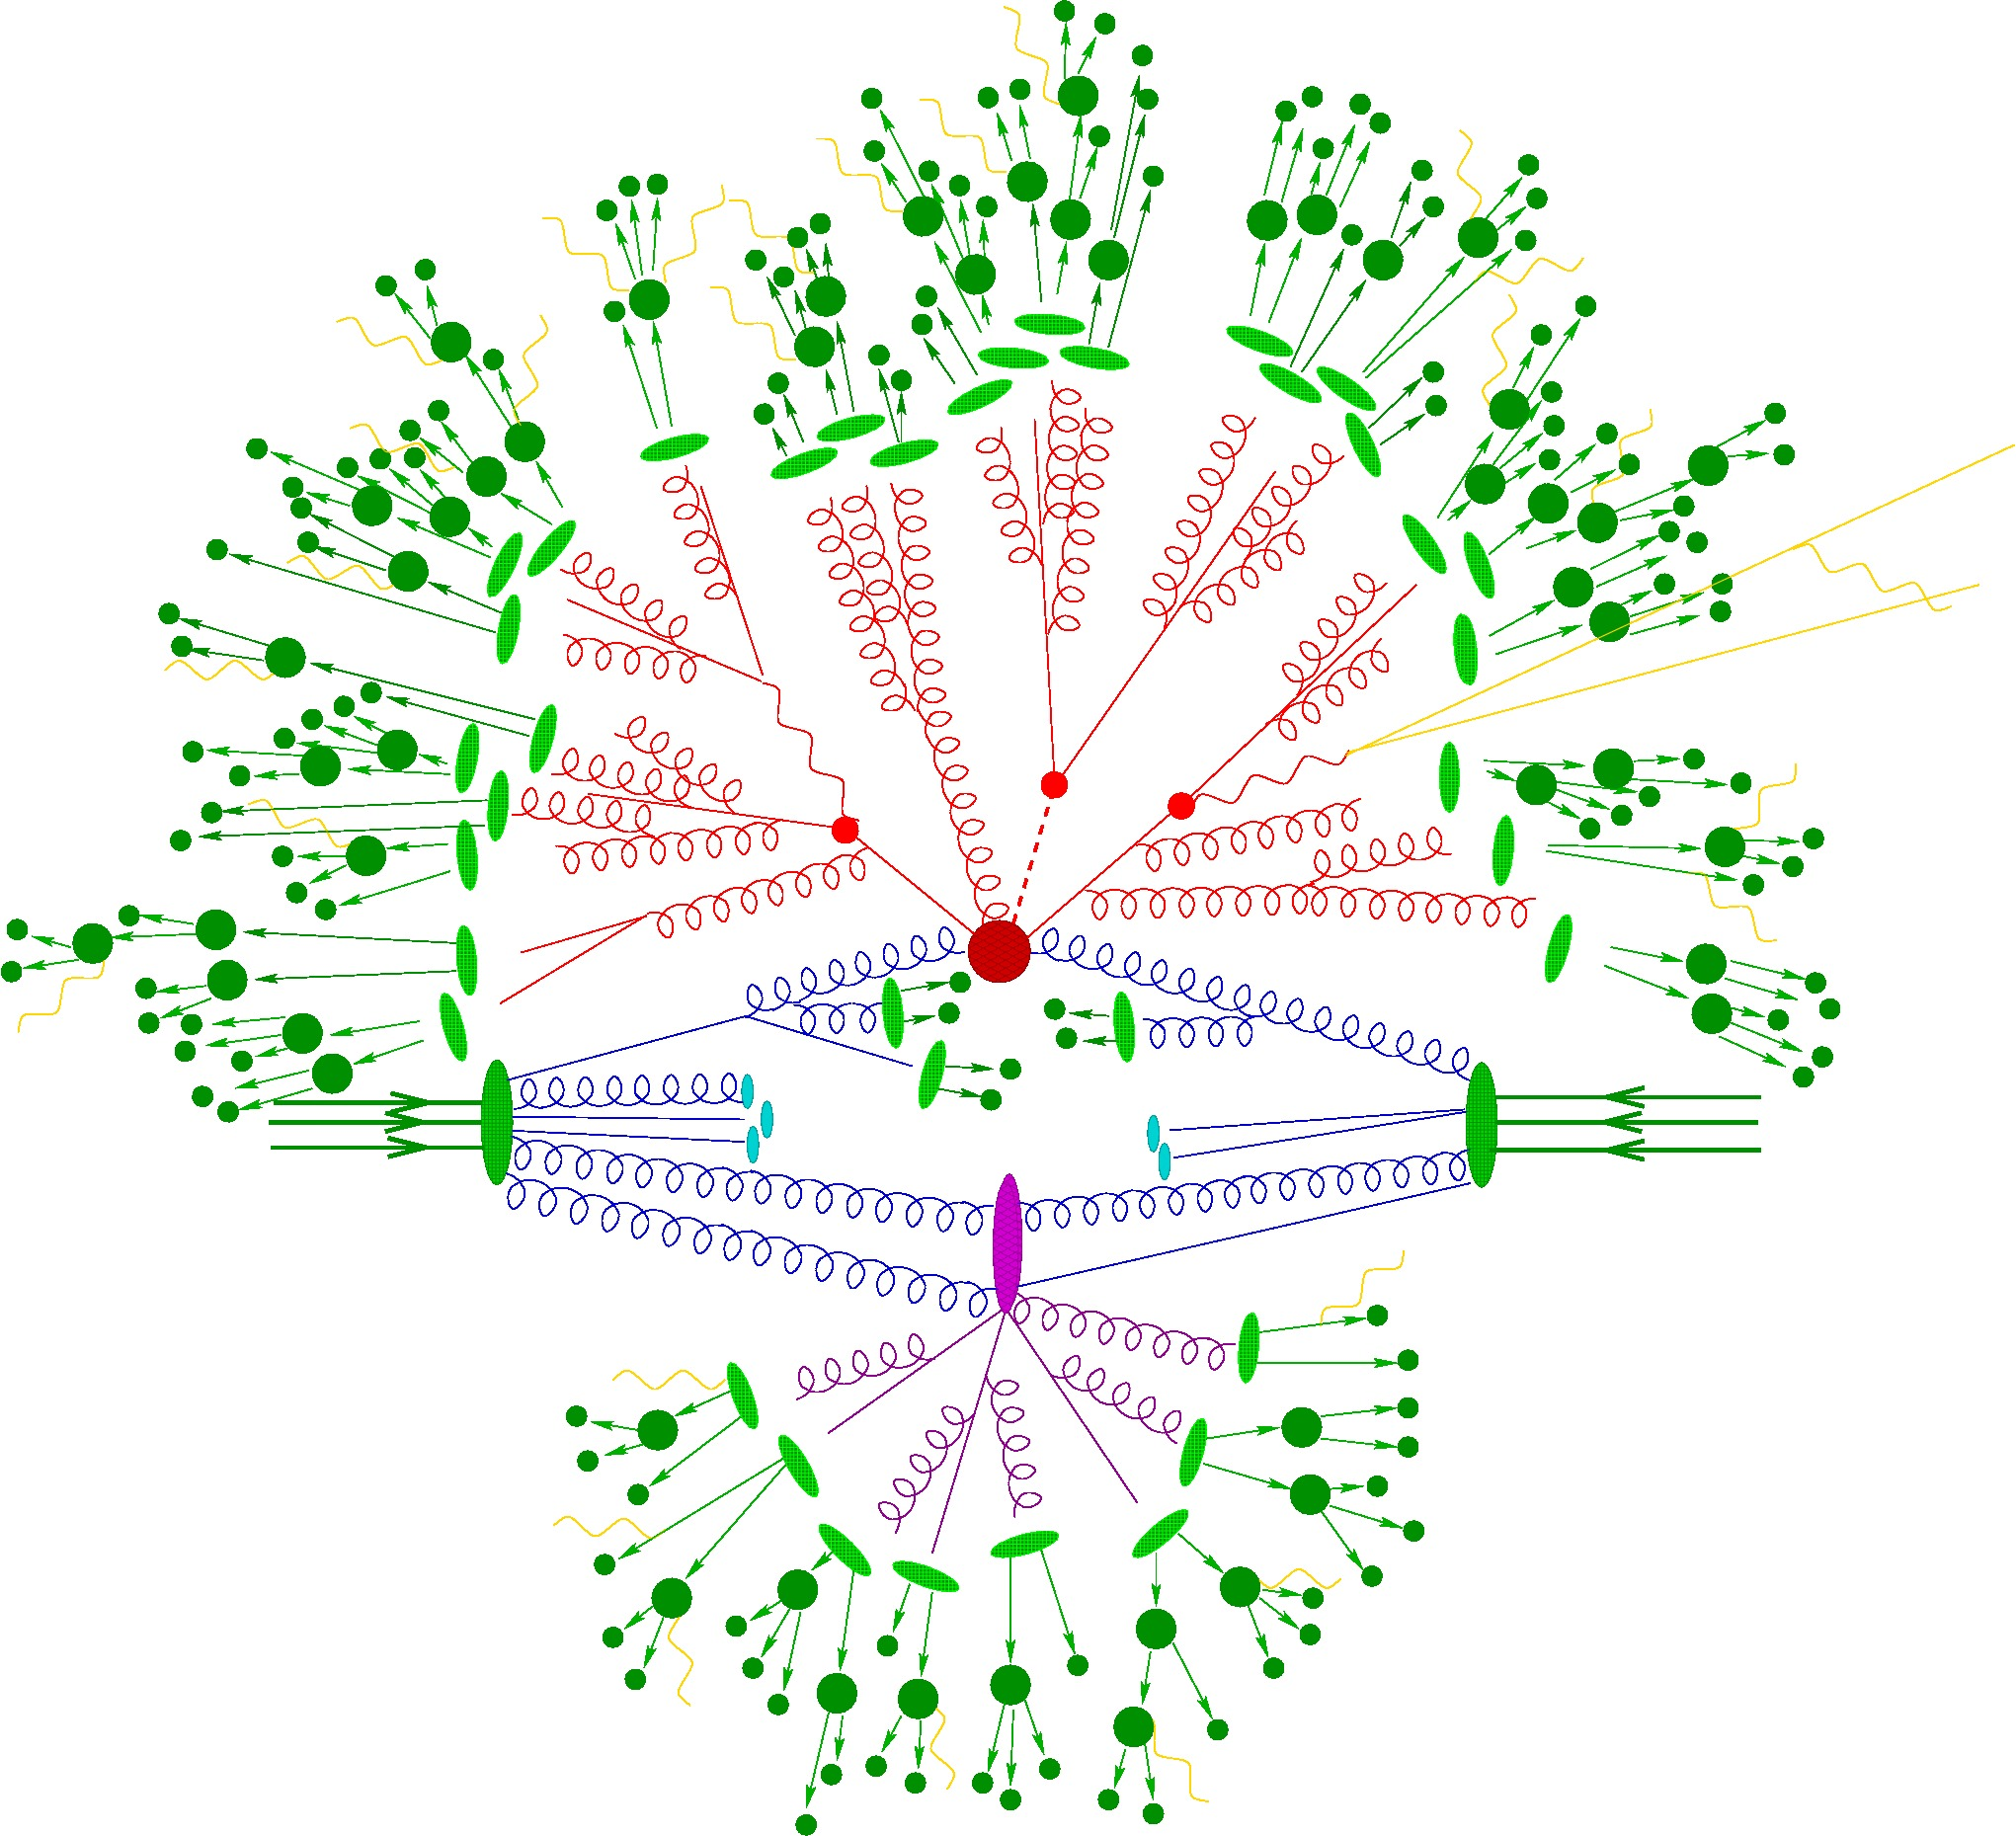
\includegraphics[width=0.8\textwidth]{figures/eventreco_event/full_event}
  \caption{Pictorial representation of a $\Pp\Pp$ collision event.
The hard interaction (big red blob) is followed by the decay of the produced particles (small red
blobs).
Additional hard QCD radiation is produced (red) and a secondary interaction takes place (purple
blob) before the final-state partons hadronize (light green blobs) and hadrons decay (dark green
blobs). Photon radiation occurs at any stage (yellow). Figure taken from
Ref.~\cite{Gleisberg:2008ta}
  \label{fig:event_full_event}}
\end{figure}


The process that is usually of most interest is the interaction between the constituents of the two
protons that results in high \pt particles. This is referred to as the \textit{hard interaction}. 
Not every collision produces very hard particles, sometimes protons merely undergo elastic
collisions, resulting in very soft scattering products that do not pass the detection thresholds. In
general, any interaction producing some detectable particles is called a \textit{minimum bias
interaction}~\cite{Field:2012jv}. 

The initial momentum distribution of the partons involved in the hard interaction is contained
within \textit{parton distribution functions} (PDFs) describing the structure of the proton. 
Apart from the hard interaction, the other constituents of the proton can also interact. This
usually results in a spray of softer particles, the \textit{underlying event} (UE). 
Any high momentum particle produced in the collision will emit additional hard QCD radiation, the
so-called initial- and final-state-radiation (ISR or FSR).

Quarks and gluons produced in the collision cannot stay free, they must hadronize in a time scale
of $\mathcal{O}(\text{10}^{\text{-23}}\second)$. These hadrons, in addition to possible produced
leptons, will then pass through the experiment where they can be detected, and used to find out
what happened in the collision itself. 
A complication for the physicists analyzing the data arises from the very high
instantaneous luminosity at the LHC. During one bunch crossing there are usually up to 20
$\Pp\Pp$ interactions, collectively referred to as \textit{pileup}. Most of these interactions
produce relatively soft particles, but they do add to the overall hadronic activity in an event,
and can obscure the interesting hard process. 
An example of how an event might look like in the CMS detector is shown in
Fig.~\ref{fig:event_display}. 

In the next subsections I will elaborate on how to describe an event in a more mathematical way,
starting from the factorization theorem. These sections are largely based on
Refs.~\cite{Campbell:2006wx,Skands:2011pf,Salam_Bautzen,Salam:2010zt,Tung:2001cv}.

\begin{figure}[htpb]
  \centering
  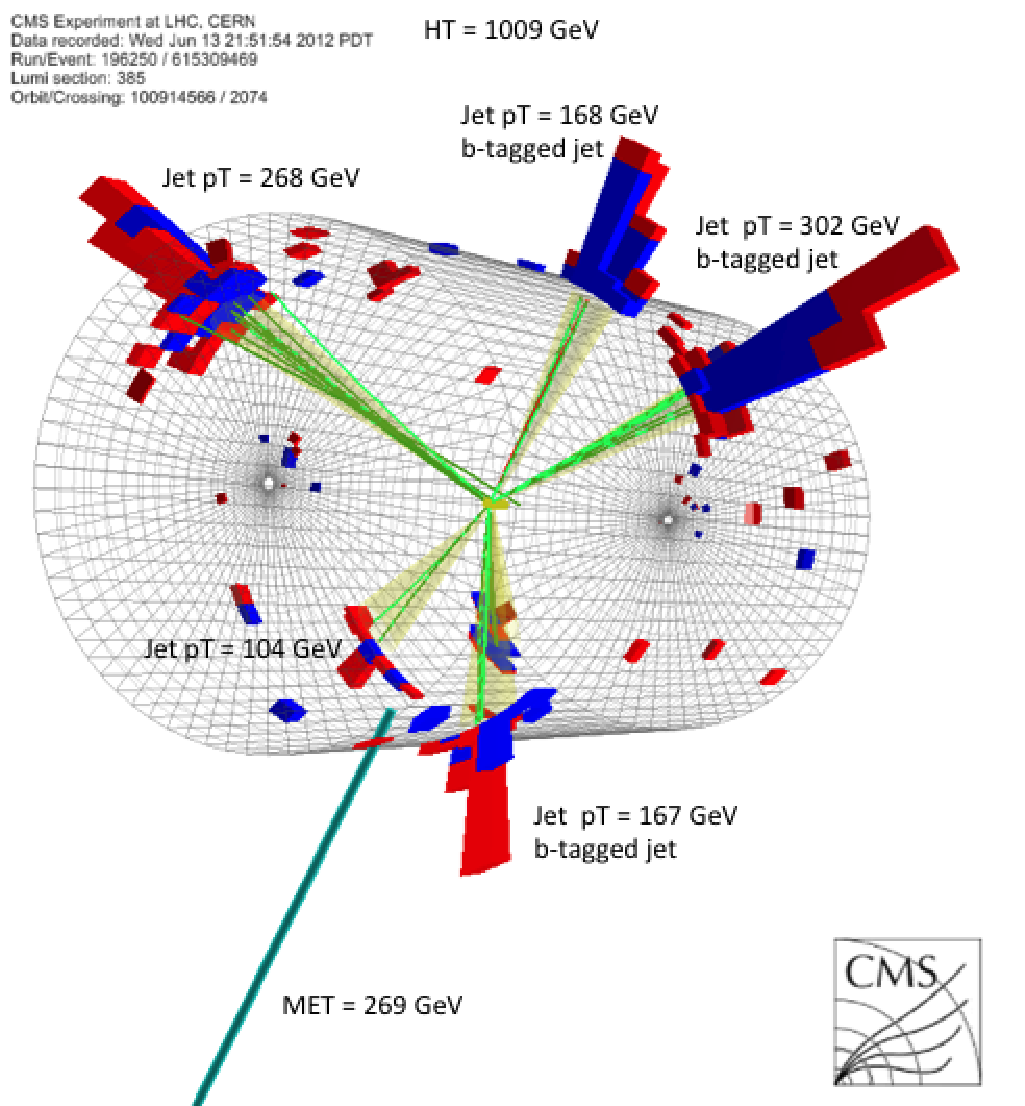
\includegraphics[width=0.7\textwidth]{figures/eventreco_event/event_display_SUS12024}
  \caption{CMS event display showing five high \pt jets, three of which are tagged as coming from a
$\cPqb$ quark. Figure from~\cite{SUS12024_event_display}.
  \label{fig:event_display}}
\end{figure}


\subsection{Factorization theorems}

The basic problem addressed by factorization theorems~\cite{Collins:1989gx} is how to calculate
cross sections for high energy processes. In general, these cross sections are a combination of
short- and long-distance contributions, and are thus not computable directly in QCD perturbation
theory.
Factorization theorems allow us to derive predictions for these cross sections,
by separating (factorizing) long-distance from short-distance effects. 
The non-perturbative long-range effects are encapsulated into the parton distribution functions
describing the distribution of partons in a hadron. 
These functions can be measured experimentally, see  Section~\ref{sec:event_pdfs}, and most
importantly the same functions can be used for different processes. 
The short-distance hard-scattering cross section can be calculated with perturbation theory
because the QCD coupling strength is small at short distances. 

The factorization theorem applied to the cross section $\sigma$ of a hard scattering initiated by
two hadrons $A$ and $B$, illustrated on Fig.~\ref{fig:event_hard_scatter},
can be expressed in terms of the parton distribution functions $f$, and partonic cross section
$\hat{\sigma}$:
\begin{multline}
  \sigma(s;\alpha_S,\mu_F,\mu_R) = \\ 
  \sum_{a,b} \int_0^1 dx_a \int_0^1 dx_b \,  f_{a/A}(x_a, \alpha_S, \mu_F) \cdot f_{b/B}(x_b,
\alpha_S, \mu_F) \cdot \hat{\sigma}(\hat{s};\alpha_S,\mu_F,\mu_R),
\label{eq:factorization_theorem} 
\end{multline}
 \begin{wrapfigure}{r}{0.4\textwidth}
  \centering
  \vspace{-1eM}
  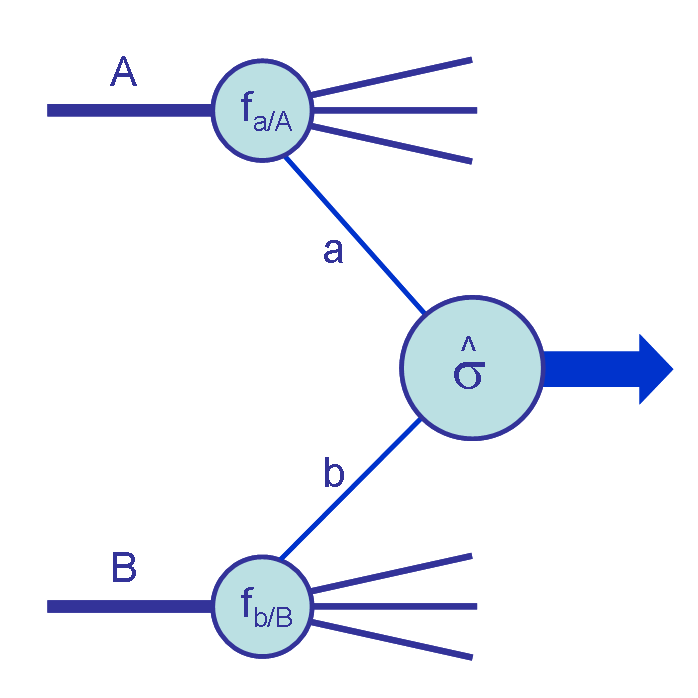
\includegraphics[width=0.38\textwidth]{figures/eventreco_event/Hardscattering}
  \caption{Diagram of a hard scattering process, showing the parton distribution functions
$f$ and the partonic cross section $\hat{\sigma}$. Figure taken from Ref.~\cite{Campbell:2006wx}.
  \label{fig:event_hard_scatter}}
\end{wrapfigure}
with $f_{a/A}(x_a, \alpha_S, \mu_F)$ the probability that a parton $a$ inside
a hadron $A$ carries a momentum fraction $x_a$, $s$ the centre-of-mass energy of the collision,
and $\hat{s} = s x_a x_b$ the partonic centre-of-mass energy.
The strong coupling constant is denoted by $\alpha_S$, the factorization scale by $\mu_F$ and the
 renormalization scale by $\mu_R$.
The factorization scale defines the (arbitrary) boundary between what is viewed as a short-range
versus a long-range interaction. The renormalization scale is also an arbitrary scale, which is
needed to regulate the divergencies that appear when computing the partonic cross section in a
perturbative expansion. 
Often, the choice $\mu_F = \mu_R$ is made for convenience.
The left-hand side of the equation is in reality independent of the arbitrary choices for $\mu_F$
and $\mu_R$. When making computations, a dependence can be introduced because we cannot
compute the partonic cross sections up to all orders in $\alpha_S$. 

The validity of this factorization theorem can be proven mathematically for certain classes of
processes (it is only approximately true for many other processes), but can also be understood
intuitively in the context of the parton model. 
Hadrons are viewed as composite objects, made up of partons held together by their interactions in
a virtual partonic state.
Let's consider how a hadron-hadron scattering at high energy and momentum transfer looks like in the
centre-of-mass frame. The hadrons appear Lorentz contracted in the direction of the collision, and
their internal interactions are time dilated. The higher the centre-of-mass energy, the longer the
lifetime of any virtual partonic state will be, and the shorter the time needed for a parton of one
hadron to cross the other hadron. At high enough energy, the time needed to traverse the hadron
will be much shorter than the lifetime of any partonic state. Each parton inside the hadron can
thus be viewed as carrying a definite fraction $\xi$ of the hadron's momentum in the centre-of-mass
frame, and so it makes sense to talk about the partons interacting rather than the hadrons.  
Therefore, the interactions of the partons inside a hadron, which occur at time-dilated time
scales before or after the hard scattering, cannot interfere with the interaction of a parton
from one hadron with a parton from the other hadron. 
The cross section for hadron scattering may thus be computed by
combining probabilities, rather than amplitudes, and factorization is reached. 




\subsection{Parton distribution functions \label{sec:event_pdfs}}

A key ingredient to the computation of any cross section at the LHC, is the set of parton
distribution functions describing the structure of the proton, as
is visible from Eq.~\ref{eq:factorization_theorem}. 
Physically, PDFs express the fact that hadrons are composite objects, with a time-dependent
structure. The PDFs themselves are not physical observables, but rather a more fundamental quantity
derived from the actual physical observables such as structure functions, which can be measured
in e.g. deep-inelastic scattering processes. 
Parton distribution functions can be extracted from this data, but only within a specific
factorization scheme, order by order in perturbation theory. 
At leading order they have a very simple physical interpretation: if the PDF for a given particle
species $p$ is given by $p(x,Q^2)$, then $p(x,Q^2) dx$ is the probability that a probe of
virtuality $Q^2$ will find a particle of flavour $p$ inside the proton, with a
momentum fraction between $x$ and $x + dx$ of the full proton momentum. 
At higher orders, the PDFs no longer have a clear probabilistic interpretation. 


Parton distribution functions satisfy sum rules, governed by the valence content of the
hadrons. For a proton we find for the PDFs of the $u$, $d$,
and $s$ (anti-)quarks: 
\begin{align}
  \int_0^1 dx \left( u(x,Q^2) - \bar{u}(x,Q^2)\right) &= 2, \\[-2pt]
  \int_0^1 dx \left( d(x,Q^2) - \bar{d}(x,Q^2)\right) &= 1, \\[-2pt]
  \int_0^1 dx \left( s(x,Q^2) - \bar{s}(x,Q^2)\right) &= 0, 
\end{align}
while we also need to satisfy that the momentum weighted sum of the PDFs of all particle species is
equal to unity, in order to satisfy momentum conservation, 
\begin{equation}
  \int_0^1 dx \, x \left( g(x,Q^2) + \sum_i [u_i(x,Q^2) + \bar{u}_i(x,Q^2)]\right) = 1 ,
\end{equation}
where $g(x,Q^2)$ is the gluon PDF, and $i$ runs over all quark flavours. 

Looking back to Eq.~\ref{eq:factorization_theorem}, we note that the parton distribution
functions depend on the chosen factorization scale. The dependence of the PDFs on the scale $Q^2$
is described by the DGLAP equations, which can be viewed as renormalization group equations in
analogy with the running coupling constant. 
The DGLAP equations, and thus the PDF evolution, are governed by the so-called splitting functions,
$P_{ab}$ , that model the rate for a particle of type $a$ to undergo a collinear splitting to
produce a particle of type $b$. 

Parton distribution functions are obtained from global fits to a wide variety of data from
many experiments, among which are measurements of deep-inelastic scattering at HERA, and Drell-Yan
or inclusive jet production at the Tevatron and the LHC. 
Since there is only a partial kinematic overlap between this data and the region in $(x,Q^2)$ space
where we want to use the PDFs, for example to model the production of supersymmetric particles,
the DGLAP evolution is essential for the successful prediction of PDFs in the LHC domain. 
The splitting functions are now known up to NNLO precision, which reduced the uncertainties on the
evolution dramatically, from 30\% down to about 2\%.

As illustration of the PDF scale dependence, we show in Fig.~\ref{fig:NNPDF} the full
set of parton distribution functions for two $Q^2$ scales, as derived by the \textsc{NNPDF}
collaboration~\cite{Ball:2012cx}. 
The gluon PDF is seen to dominate for small momentum fractions, and this domination increases as the
scale increases. This simply means that as we probe the proton with higher energy, i.e. to smaller
length scales, we will find more and more gluons. 

\begin{figure}[tpb]
  \centering
  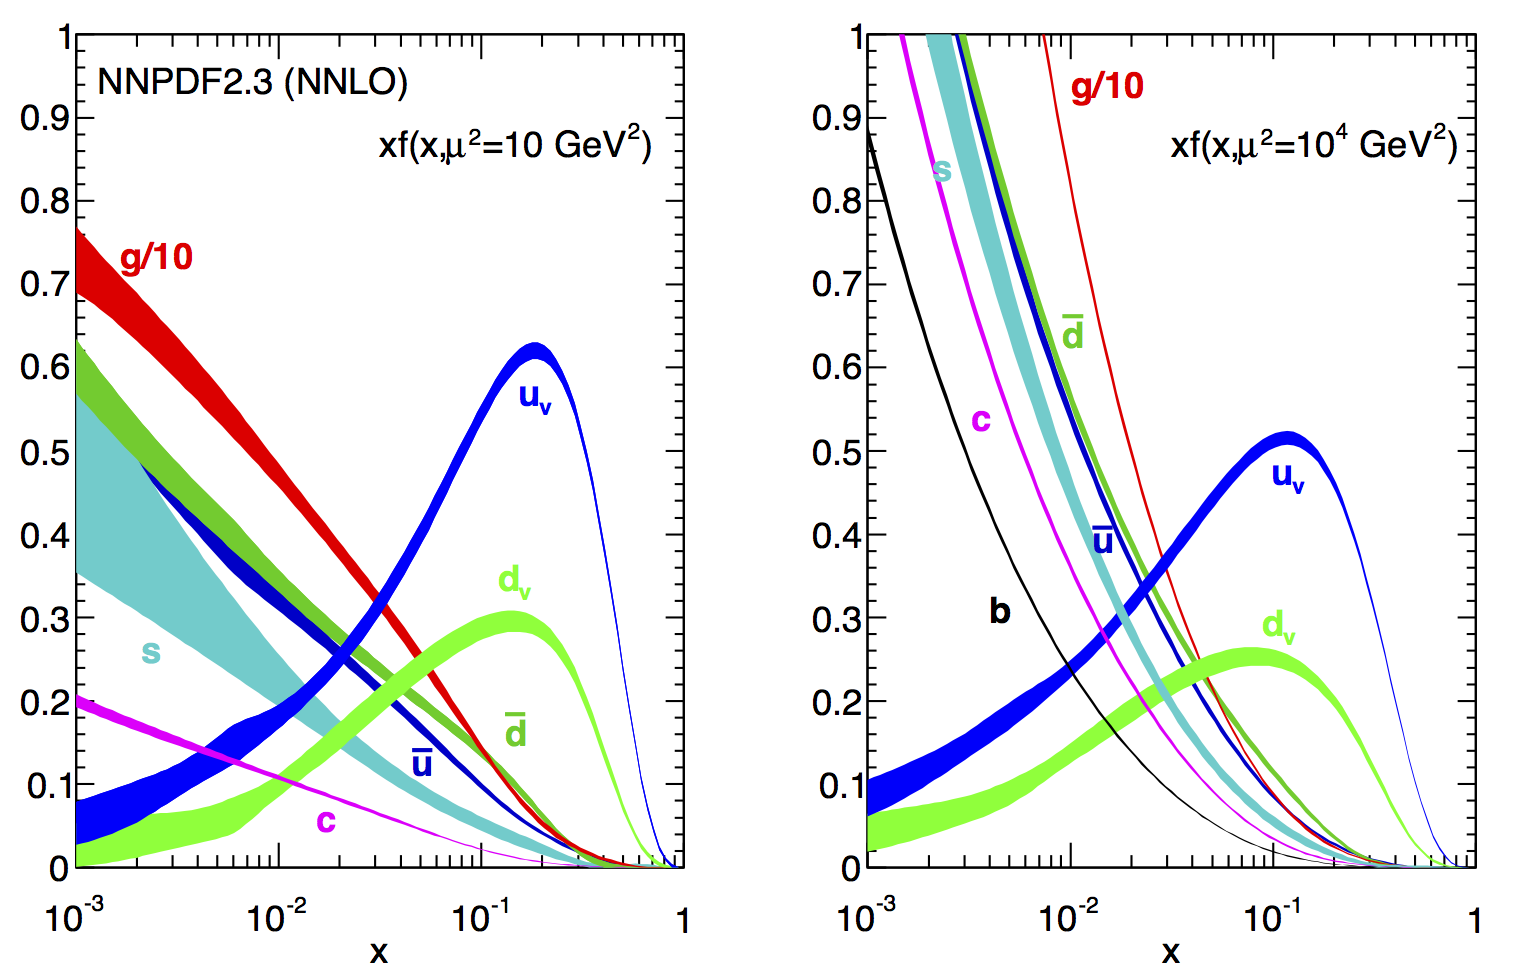
\includegraphics[width=0.8\textwidth]{figures/eventreco_event/nnpdf23_nnlo_allpdfs}
  \caption{Parton distribution functions for different parton species inside the proton for two
values for the momentum transfer, as obtained by the \textsc{NNPDF}
collaboration~\cite{NNPDF_website,Ball:2012cx}. 
  \label{fig:NNPDF}}
\end{figure}

Most global analyses, such as the one performed by the \textsc{CTEQ} or \textsc{MSTW}
collaborations, use a generic form for the parameterization of the quark and gluon distributions at
some reference value $Q_0$, usually chosen in the range $1-2\GeV$:
\begin{equation}
  f(x,Q_0) = A_0 x^{A_1} (1-x)^{A_2} P(x; A_3, \ldots) .
\end{equation}
The parameter $A_1$ is associated with small-$x$ behaviour, while $A_2$ is associated with
large $x$. These two factors are, in general, not sufficient to describe the quark or gluon
distribution functions. The term $P(x; A_3, \ldots)$ is a smooth function, depending on one or more
parameters, that is introduced to add more flexibility to the PDF parameterization. The various PDF
collaborations usually make different choices for the form of $P(x)$. 
The coefficients $A_i$ are then usually determined by comparing theoretical predictions with the
data using the method of least-$\chi^2$ fits. 
The \textsc{NNPDF} collaboration uses a different approach, and parameterizes $f(x,Q_0)$ by a
neural network. 
Once the PDFs are determined for the reference value $Q_0$, they are generated for the full
$(x,Q^2)$ plane using the DGLAP evolution equations. 

Apart from having an estimate for the nominal values of the PDFs in a given kinematic range, it is
also important to understand the uncertainties, especially for the gluon PDF, which is the hardest
to access experimentally, and is constrained mostly by the $Q^2$ evolution of the quark PDFs. 
A common method of estimating parton distribution uncertainties is to compare different published
parton distributions. This poses a problem since most published PDF sets adopt similar
assumptions such that the differences between these sets do not fully capture the uncertainties that
actually exist. Several techniques exists that remedy this, and they are used by the PDF
collaborations to publish a proper set of uncertainties with each PDF set.  



\subsection{Hard interaction \label{sec:event_hard_interaction}}

% mention following things:
% - complications arising from MPI
% - make link to section on matrix element generators which will contain more info on the practical
% implementation


The partonic scattering cross section describes the hard interaction, and contains all the
short-range effects. For the interaction between two partons $a$ and $b$, resulting in final state
$F$ plus anything else ($X$), it can be written as
\begin{equation}
  \hat{\sigma}_{ab\rightarrow F+X} = \frac{1}{2\hat{s}_{ab}} | \mathcal{M}_{ab\rightarrow
F+X}|^2(\Phi_F, \mu_F, \mu_R), 
\end{equation}
with $\hat{s} = (p_a + p_b)^2$ the usual Mandelstam variable, and 
$|\mathcal{M}|^2$ the matrix element squared for the process $a b \rightarrow F+X$, appropriately
summed and averaged over the relevant helicities and colours. 
The matrix element depends on the final state phase space $\Phi_F$, and should be evaluated at the
factorization scale $\mu_F$ and renormalization scale $\mu_R$.

The partonic cross section can be expanded in a perturbative series in the strength of the
QCD coupling constant $\alpha_S$, 
\begin{equation}
  \hat{\sigma} = \hat{\sigma}_0 + \hat{\sigma}_1 \alpha_S + \hat{\sigma}_2 \alpha_S^2 + \ldots
\end{equation}
The first couple of terms in the perturbative expansion are the terms that so-called
\textit{fixed-order predictions} deal with. They are conceptually quite simple; it is easy to state
which contributions are included, and by including further orders in the expansion one can expect to
see improvement in the accuracy of the predictions. 
At leading order we can still compute many inclusive cross sections by hand, although this is often
automated, by computing all the relevant tree-level Feynman diagrams and integrating over the
appropriate phase space. 
At next-to-leading order we can distinguish between two sets of extra contributions to the
originally considered process: the real emissions resulting in extra quarks or gluons in the final
state, and the virtual loops which do not change the number of final state particles, but do impact
the cross section. 

It is important to note that the complexity of the computations increases mostly with the number of
extra loops, rather than the actual order in $\alpha_S$. 
Tree-level diagrams can be calculated up to quite high final-state multiplicities, $\sim\,$10,
while one-loop diagrams have only been used for processes with up to 3 or sometimes 4 final-state
particles, and two-loop diagrams are available only for $2 \rightarrow 1$ type processes, such as
$\Pp\Pp \rightarrow W$.
When going to higher orders in the perturbative series, it also becomes more and more tricky to
properly combine, i.e. cancel, divergencies between 2-loops, 1-loop and tree-level diagrams. 
Examples of tree-level diagrams that become divergent is anything produced in association with
extra quarks or gluons which could become soft or collinear. These divergencies must be cancelled
by the corresponding loop divergencies, otherwise unitarity is violated. 
In practice this is not always easy to do, especially when experimental cuts need to be applied. 
The standard technique to deal with this issue is through a \textit{subtraction procedure} which
introduces suitable counterterms, adding them to the real diagrams, and subtracting them from the
loops, hereby removing the divergencies from the calculation.


Even though the switch from LO to NLO predictions introduces some technical complications, it is
still worthwhile to do so, where possible, because of the reduced uncertainties. 
At NLO, the dependence on the factorization and renormalization scales is much smaller, as this
relies on the missing higher order terms, which for NLO contain an extra factor $\alpha_S$, and are
thus smaller.

The strength of the NLO correction is often encapsulated in a so-called NLO k-factor, which is
defined as the ratio of the NLO cross section to the LO cross section. K-factors for many processes
can be as large as 1.5, much larger than the 10\% effect one would expect from considering only the
extra factor of $\alpha_S$. The reason for this is that the terms accompanying that factor of
$\alpha_S$ can be quite large. 
The calculated k-factors can vary for different kinematic regimes within the same process, so care
needs to be taken when attempting to scale a LO cross section obtained for some particular corner of
phase space. 


As explained in the introduction of this chapter, we also need to generate full events for
which we can simulate the detector response, rather than only computing inclusive cross sections.
This chain often starts by generating events for the hard process only, of course taking into
account the parton distribution functions as well. 
Until recently, event generators based on the perturbative calculation of matrix elements could only
generate events up to LO. 
With the release of \textsc{MG5\_aMC@NLO}~\cite{Alwall:2014hca}, the automated generation of events
at NLO precision is now possible for almost any Standard Model process.
More details on how this is done in practice are presented in
Section~\ref{sec:event_matrix_element_generators}.



